\documentclass[tikz, border=4pt]{standalone}
\usepackage[T1]{fontenc}
\usepackage{lmodern}
\usepackage{amssymb}
\usetikzlibrary{positioning, calc, fit, backgrounds, arrows.meta, matrix}

% Candidate frameworks as sets of functions: the approach, drawn on four real
% assumptions of the corpus (CKM_84, CKM_04, CKM_43, CKM_52) under the reference
% specification. Step 1: each assumption serves a set of functions. Step 2: a
% framework is a set of functions and captures an assumption only if it measures
% every function the assumption serves. Step 3: for each width k, among all sets
% of k functions, keep the one that captures the largest share of assumptions.
% Shares in step 3 are the reference specification (code/61).

\definecolor{leg}{HTML}{2166ac}
\definecolor{irr}{HTML}{b2182b}
\definecolor{band}{HTML}{dbe6f2}

\begin{document}
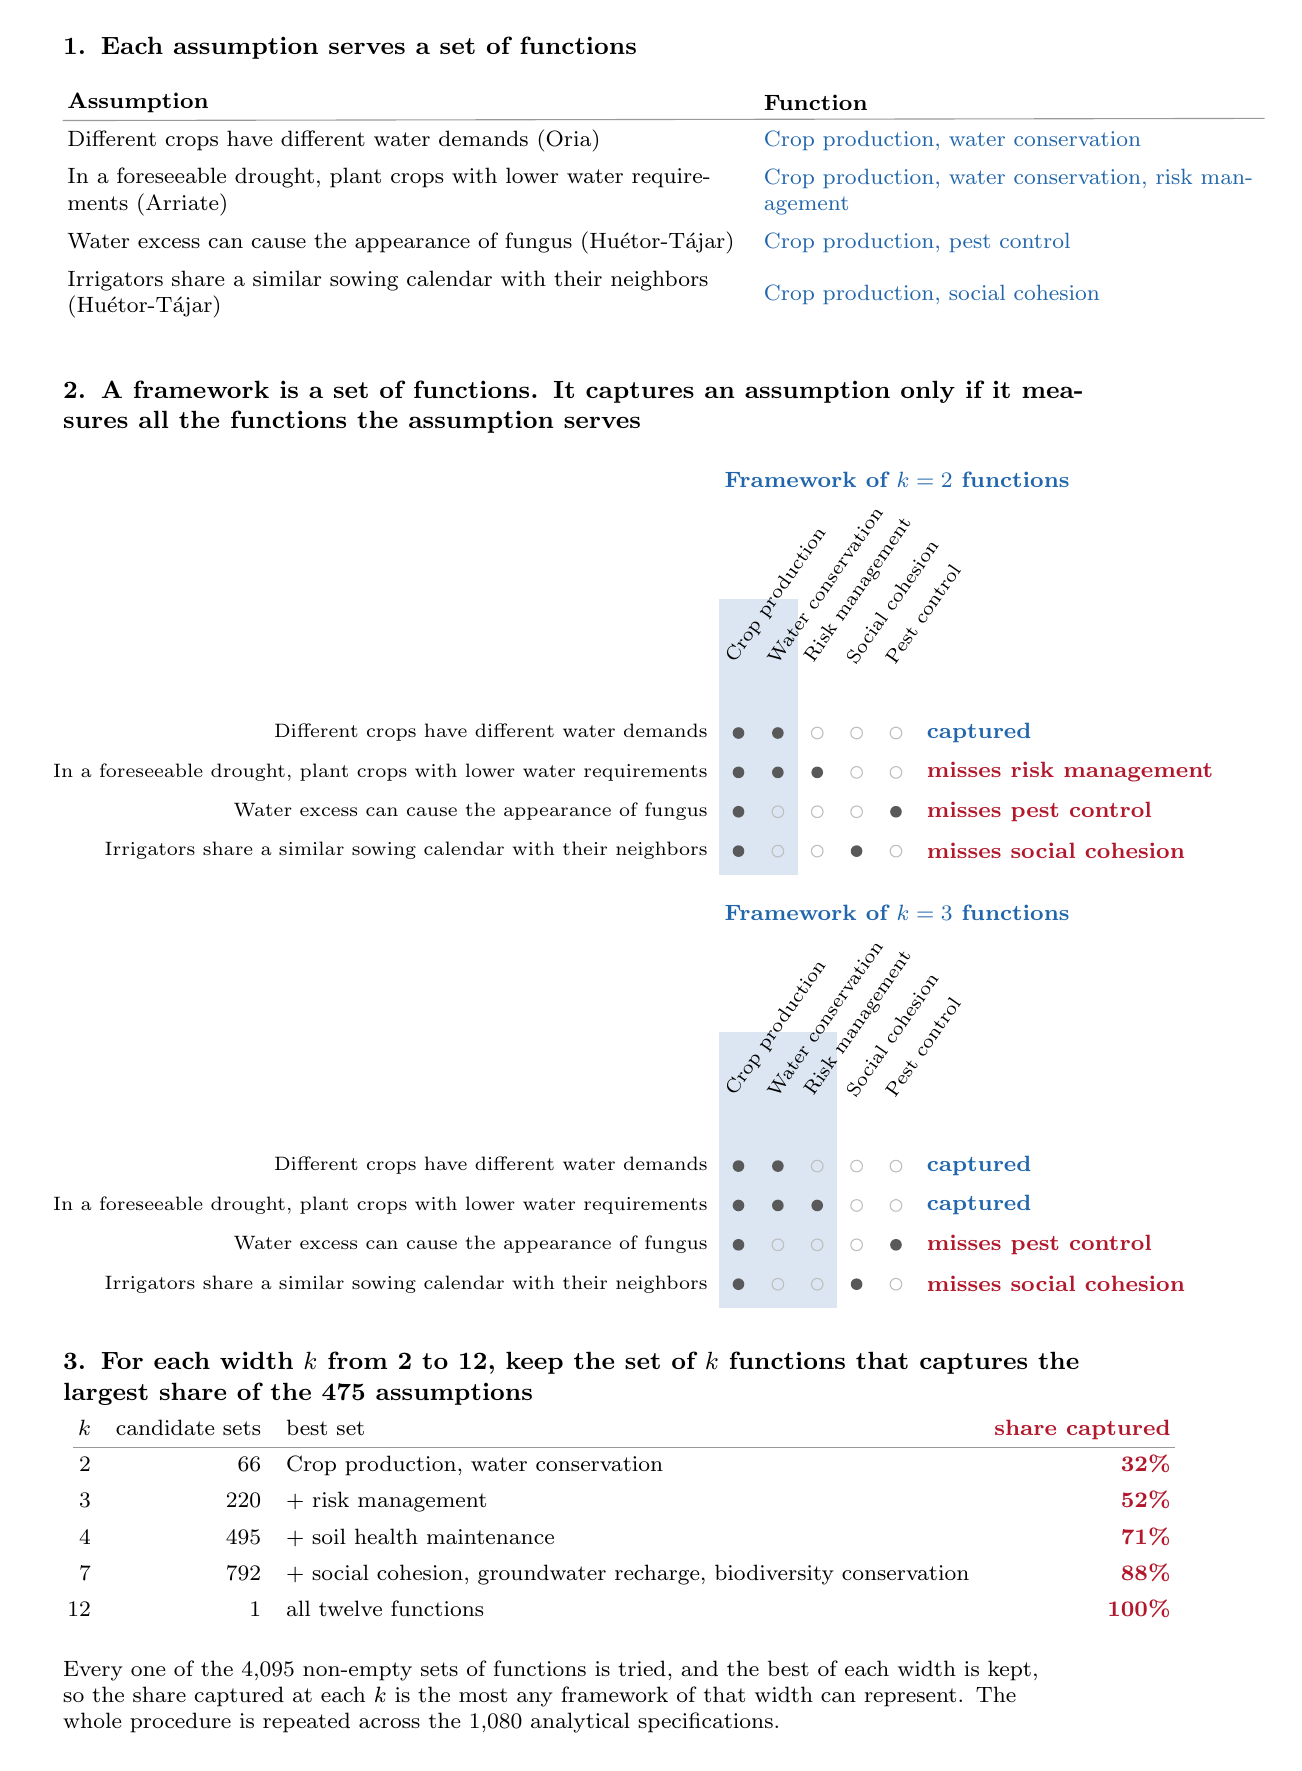
\begin{tikzpicture}[
  font=\footnotesize,
  dot/.style={circle, fill=black!65, inner sep=0pt, minimum size=4.2pt},
  nodot/.style={circle, draw=black!25, inner sep=0pt, minimum size=4.2pt},
  head/.style={rotate=55, anchor=south west, inner sep=1pt, font=\scriptsize},
  stp/.style={font=\bfseries\small, anchor=west, text width=13.5cm, align=left},
  note/.style={font=\footnotesize, text width=12.5cm, align=left},
  rlab/.style={anchor=east, inner sep=1pt, text width=8.6cm, align=right, font=\scriptsize},
  yes/.style={text=leg, font=\footnotesize\bfseries, anchor=west, inner sep=1pt},
  no/.style={text=irr, font=\footnotesize\bfseries, anchor=west, inner sep=1pt},
]

% ----------------------------------------------------------------------------
% Step 1: assumptions and the functions they serve
% ----------------------------------------------------------------------------

\node[stp] (s1) at (-4.1, 0) {1. Each assumption serves a set of functions};

\matrix (A) [matrix of nodes, below=4mm of s1.west, anchor=north west,
             row sep=3pt, column sep=4pt,
             nodes={anchor=west, inner sep=1.5pt},
             row 1/.style={nodes={font=\footnotesize\bfseries, text=black}},
             column 1/.style={nodes={text width=8.6cm, align=left}},
             column 2/.style={nodes={text width=6.3cm, align=left}}] {
  Assumption & Function \\
  Different crops have different water demands (Oria) & {\color{leg}Crop production, water conservation} \\
  In a foreseeable drought, plant crops with lower water requirements (Arriate) & {\color{leg}Crop production, water conservation, risk management} \\
  Water excess can cause the appearance of fungus (Hu\'etor-T\'ajar) & {\color{leg}Crop production, pest control} \\
  Irrigators share a similar sowing calendar with their neighbors (Hu\'etor-T\'ajar) & {\color{leg}Crop production, social cohesion} \\
};
\draw[black!40] ($(A-1-1.south west)+(0,-1pt)$) -- ($(A-1-2.south east)+(0,-1pt)$);

% ----------------------------------------------------------------------------
% Step 2: a framework is a set of functions; it captures an assumption only if
% it measures all the functions the assumption serves
% ----------------------------------------------------------------------------

\node[stp, below=5mm of A.south west, anchor=north west] (s2)
  {2. A framework is a set of functions. It captures an assumption only if it measures all the functions the assumption serves};

% Two incidence grids: the same four assumptions against five functions, with
% the framework's columns shaded. Columns: Crop, Water, Risk, Social, Pest.

\newcommand{\grid}[4]{% name, x, y, number of shaded columns
  \begin{scope}[shift={(#2, #3)}]
    \begin{scope}[on background layer]
      \fill[band] (-0.25, -2.3) rectangle (#4*0.5 - 0.25, 1.2);
    \end{scope}
    \foreach \lab [count=\i from 0] in {Crop production, Water conservation,
                                        Risk management, Social cohesion, Pest control}
      \node[head] at (\i*0.5, 0.3) {\lab};
    % assumption 1: crop, water
    \node[dot] at (0, -0.5) {}; \node[dot] at (0.5, -0.5) {};
    \node[nodot] at (1, -0.5) {}; \node[nodot] at (1.5, -0.5) {}; \node[nodot] at (2, -0.5) {};
    % assumption 2: crop, water, risk
    \node[dot] at (0, -1) {}; \node[dot] at (0.5, -1) {}; \node[dot] at (1, -1) {};
    \node[nodot] at (1.5, -1) {}; \node[nodot] at (2, -1) {};
    % assumption 3: crop, pest
    \node[dot] at (0, -1.5) {}; \node[nodot] at (0.5, -1.5) {}; \node[nodot] at (1, -1.5) {};
    \node[nodot] at (1.5, -1.5) {}; \node[dot] at (2, -1.5) {};
    % assumption 4: crop, social
    \node[dot] at (0, -2) {}; \node[nodot] at (0.5, -2) {}; \node[nodot] at (1, -2) {};
    \node[dot] at (1.5, -2) {}; \node[nodot] at (2, -2) {};
    \node[rlab] at (-0.35, -0.5) {Different crops have different water demands};
    \node[rlab] at (-0.35, -1) {In a foreseeable drought, plant crops with lower water requirements};
    \node[rlab] at (-0.35, -1.5) {Water excess can cause the appearance of fungus};
    \node[rlab] at (-0.35, -2) {Irrigators share a similar sowing calendar with their neighbors};
    \coordinate (#1-tl) at (-0.25, 0.25);
    \coordinate (#1-br) at (2.25, -2.3);
  \end{scope}
}

\grid{G2}{4.6}{-8.2}{2}
\node[yes] at (6.95, -8.7) {captured};
\node[no]  at (6.95, -9.2) {misses risk management};
\node[no]  at (6.95, -9.7) {misses pest control};
\node[no]  at (6.95, -10.2) {misses social cohesion};
\node[anchor=south west, text=leg, font=\footnotesize\bfseries] at (4.3, -5.7)
  {Framework of $k=2$ functions};

\grid{G3}{4.6}{-13.7}{3}
\node[yes] at (6.95, -14.2) {captured};
\node[yes] at (6.95, -14.7) {captured};
\node[no]  at (6.95, -15.2) {misses pest control};
\node[no]  at (6.95, -15.7) {misses social cohesion};
\node[anchor=south west, text=leg, font=\footnotesize\bfseries] at (4.3, -11.2)
  {Framework of $k=3$ functions};

% ----------------------------------------------------------------------------
% Step 3: for each width, keep the set that captures most
% ----------------------------------------------------------------------------

\node[stp] (s3) at (-4.1, -16.9)
  {3. For each width $k$ from 2 to 12, keep the set of $k$ functions that captures the largest share of the 475 assumptions};

\matrix (B) [matrix of nodes, below=3mm of s3.west, anchor=north west,
             row sep=1.5pt, column sep=6pt,
             nodes={anchor=west, inner sep=1.5pt, text height=1.6ex, text depth=0.4ex},
             column 1/.style={nodes={anchor=east}},
             column 2/.style={nodes={anchor=east}},
             column 4/.style={nodes={anchor=east, text=irr, font=\footnotesize\bfseries}}] {
  $k$ & candidate sets & best set & share captured \\
  2  & 66    & Crop production, water conservation & 32\% \\
  3  & 220   & $+$ risk management & 52\% \\
  4  & 495   & $+$ soil health maintenance & 71\% \\
  7  & 792   & $+$ social cohesion, groundwater recharge, biodiversity conservation & 88\% \\
  12 & 1     & all twelve functions & 100\% \\
};
\draw[black!40] ($(B-1-1.south west)+(0,-1pt)$) -- ($(B-1-4.south east)+(0,-1pt)$);

\node[note, text width=12.5cm, anchor=north west] at ($(B.south west)+(0,-2mm)$)
  {Every one of the 4,095 non-empty sets of functions is tried, and the best of each
   width is kept, so the share captured at each $k$ is the most any framework of
   that width can represent. The whole procedure is repeated across the 1,080
   analytical specifications.};

\end{tikzpicture}
\end{document}
